\chapter*{ضمیمهٔ ۵: تقابل‌های موضوعی}
\addcontentsline{toc}{chapter}{ضمیمهٔ ۵: تقابل‌های موضوعی}
\markboth{ضمیمهٔ ۵: تقابل‌های موضوعی}{ضمیمهٔ ۵: تقابل‌های موضوعی}
\thispagestyle{plain}

\begin{center}
  \resizebox{\columnwidth}{!}{%
\begin{tikzpicture}
    \node[
      draw=GoldAccent, line width=1.2pt,
      fill=GoldAccent!6,
      rounded corners=6pt,
      inner sep=10pt,
      text width=0.82\linewidth,
      align=center
    ] {
      \textcolor{DarkGray}{\large\itshape
        تصویرسازی بصری از تنش‌های بنیادین اندیشهٔ سیاسی}\\[4pt]
      \textcolor{MediumGray}{\small
        هر بخش با منابع آکادمیک دست‌اول مستند شده است}
    };
  \end{tikzpicture}%
}
\end{center}

% FIXED: ornamentalrule بدون \leaders — در این موقعیت امن است
\ornamentalrule
\vspace{6pt}

% ─────────────────────────────────────────────────────────────────
\section*{۱. طیف سیاسی: اینفوگرافیک}
% ─────────────────────────────────────────────────────────────────

\begin{figure}[H]
  \centering
  % FIXED: از PDF استفاده کنید (SVG را با Inkscape تبدیل کنید)
  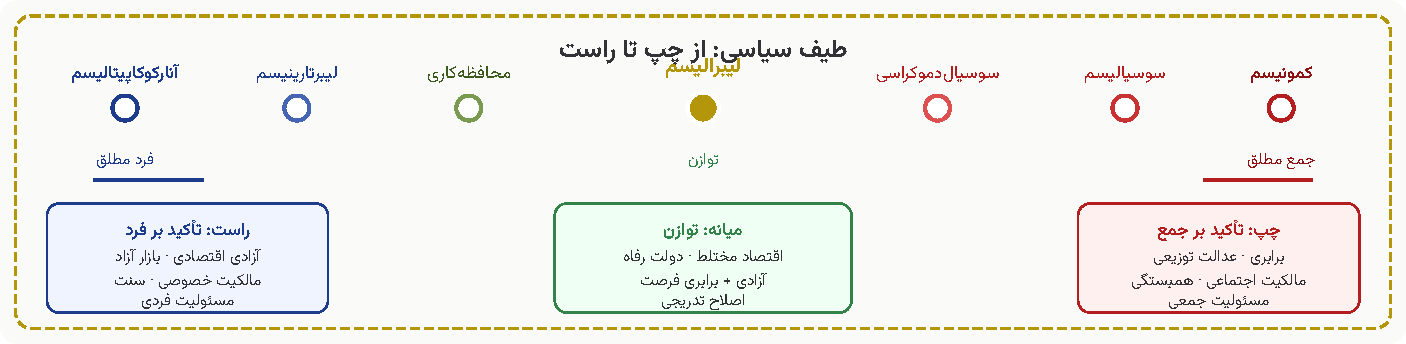
\includegraphics[width=\linewidth]{figures/infographic-spectrum.pdf}
  \caption{طیف سیاسی از آنارکو‌کاپیتالیسم تا کمونیسم}
  \label{fig:spectrum}
\end{figure}

% FIXED: rounded corners بدون مقدار
\begin{defbox}[چارچوب نظری: طیف یک‌بُعدی و محدودیت‌های آن]
تقسیم‌بندی چپ–راست از انقلاب فرانسه (۱۷۸۹) سرچشمه می‌گیرد.
\person{نولان} (۱۹۷۱) با نمودار دوبُعدی خود نشان داد این طیف خطی،
آزادی‌های شخصی را نادیده می‌گیرد.\\[4pt]
{\small\en{Bobbio, N. (1996).
\textit{Left and Right: The Significance of a Political Distinction}.
University of Chicago Press.}}
\end{defbox}

\vspace{6pt}
\ornamentalrule
\vspace{4pt}

% ─────────────────────────────────────────────────────────────────
\section*{۲. نقشهٔ دوبُعدی ایدئولوژی‌ها}
% ─────────────────────────────────────────────────────────────────

\begin{figure}[H]
  \centering
  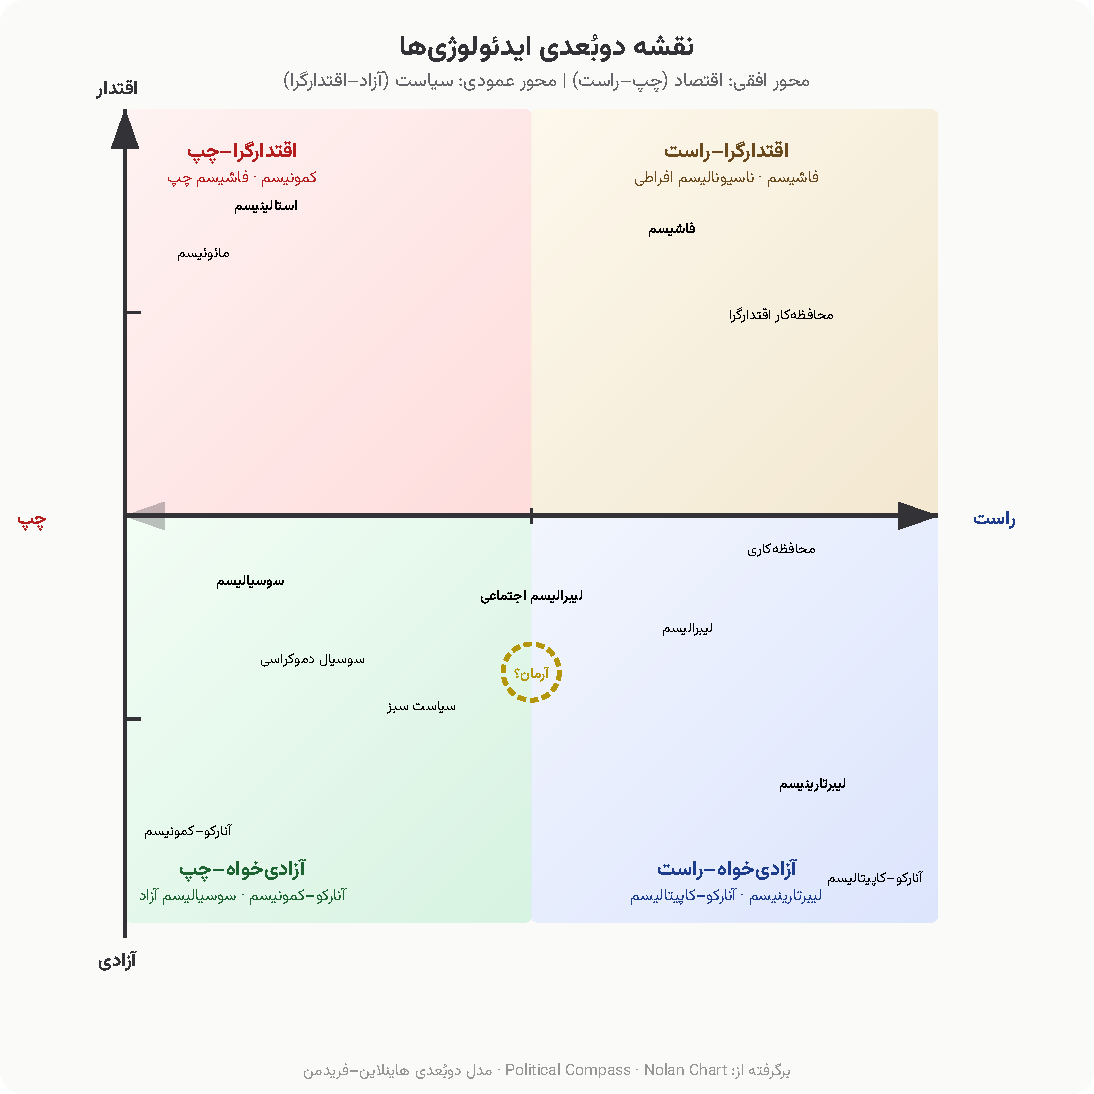
\includegraphics[width=0.92\linewidth]{figures/infographic-2axis.pdf}
  \caption{جایابی ایدئولوژی‌ها در دو محور اقتصادی و سیاسی}
  \label{fig:twoaxis}
\end{figure}

\begin{comparebox}[نمودار نولان و قطب‌نمای سیاسی]
\begin{itemize}[leftmargin=*, itemsep=3pt]
  \item \keyword{محور افقی}: اقتصاد — از مداخلهٔ کامل دولت (چپ)
        تا بازار کاملاً آزاد (راست)
  \item \keyword{محور عمودی}: سیاست — از آزادی‌های مدنی کامل (پایین)
        تا کنترل کامل دولت (بالا)
  \item \leftkw{چپ–اقتدارگرا}: استالینیسم، مائوئیسم
  \item \rightkw{راست–اقتدارگرا}: فاشیسم، ناسیونالیسم افراطی
  \item \centerkw{چپ–آزادی‌خواه}: آنارکو–کمونیسم، سوسیالیسم آزاد
  \item \rightkw{راست–آزادی‌خواه}: لیبرتارینیسم، آنارکو–کاپیتالیسم
\end{itemize}
\mediumspace
{\small\en{Nolan, D. (1971). Classifying and Analyzing
Politico-Economic Systems. \textit{The Individualist}.}}
\end{comparebox}

\ornamentalrule
\vspace{4pt}

% ─────────────────────────────────────────────────────────────────
\section*{۳. فرد در برابر جمع}
% ─────────────────────────────────────────────────────────────────

\begin{center}
\resizebox{\columnwidth}{!}{%
\begin{tikzpicture}[scale=1, every node/.style={font=\small}]

  % گرادیان رنگی با مستطیل‌های متوالی
  \foreach \i in {0,...,27} {
    \pgfmathsetmacro{\rval}{int(30 + \i*5)}
    \pgfmathsetmacro{\bval}{int(140 - \i*5)}
    \definecolor{gradcol}{RGB}{\rval,60,\bval}
    \fill[gradcol] (\i*0.5, -0.22) rectangle (\i*0.5+0.55, 0.22);
  }
  \draw[DarkGray, line width=0.8pt] (0,-0.22) rectangle (14,0.22);

  % نقطه‌های موقعیت
  \foreach \x/\col in {
      1/RightBlueDark,
      3.2/RightBlue,
      5.5/CenterGreenDark,
      7/CenterGreen,
      9/LeftRedLight,
      11.5/LeftRed,
      13/LeftRedDark}{
    \fill[\col] (\x,0) circle (5pt);
  }

  % برچسب‌های بالا
  \node[above, align=center, text width=1.8cm]
    at (1,0.3)   {\rl{آنارکو کاپیتالیسم}};
  \node[above, align=center, text width=1.8cm]
    at (3.2,0.3) {\rl{لیبرتارینیسم}};
  \node[above, align=center, text width=1.6cm]
    at (5.5,0.3) {\rl{لیبرالیسم کلاسیک}};
  \node[above, align=center, text width=1.6cm]
    at (7,0.3)   {\rl{سوسیال دموکراسی}};
  \node[above, align=center, text width=1.6cm]
    at (9,0.3)   {\rl{سوسیالیسم دموکراتیک}};
  \node[above, align=center, text width=1.4cm]
    at (11.5,0.3){\rl{سوسیالیسم}};
  \node[above, align=center, text width=1.4cm]
    at (13,0.3)  {\rl{کمونیسم}};

  % برچسب‌های قطب
  \node[below, font=\bfseries, color=RightBlue] at (1,-0.4)
    {\rl{فرد مطلق}};
  \node[below, font=\bfseries, color=LeftRed]   at (13,-0.4)
    {\rl{جمع مطلق}};
  \node[below, font=\bfseries, color=CenterGreen] at (7,-0.4)
    {\rl{توازن}};

  % باکس‌های توضیحی
  \node[draw=RightBlue, fill=RightBlue!8, rounded corners=4pt,
        align=right, text width=4.5cm] at (1.5,4) {
    \textbf{\textcolor{RightBlue}{\rl{تأکید بر فرد:}}}\\[2pt]
    \rl{• حقوق طبیعی (لاک)}\\
    \rl{• مالکیت = شخصیت (هگل)}\\
    \rl{• مسئولیت شخصی}\\
    \rl{• رقابت انتخاب اصلح}\\[2pt]
    {\footnotesize\en{Locke (1689), Nozick (1974)}}
  };

  \node[draw=CenterGreen, fill=CenterGreen!8, rounded corners=4pt,
        align=right, text width=4cm] at (7,4) {
    \textbf{\textcolor{CenterGreen}{\rl{توازن:}}}\\[2pt]
    \rl{• رولز: پرده جهل}\\
    \rl{• سندل: جماعت‌گرایی}\\
    \rl{• حقوق + وظایف}\\[2pt]
    {\footnotesize\en{Rawls (1971)}}
  };

  \node[draw=LeftRed, fill=LeftRed!8, rounded corners=4pt,
        align=right, text width=4.5cm] at (12,4) {
    \textbf{\textcolor{LeftRed}{\rl{تأکید بر جمع:}}}\\[2pt]
    \rl{• روسو: ارادهٔ عمومی}\\
    \rl{• مارکس: آگاهی طبقاتی}\\
    \rl{• همبستگی (دورکیم)}\\
    \rl{• منافع عمومی مقدم}\\[2pt]
    {\footnotesize\en{Marx (1867), Rousseau (1762)}}
  };

  % خطوط ارتباطی
  \draw[RightBlue!40, dashed, line width=0.7pt]
    (1.5,2.3) -- (1,0.3);
  \draw[CenterGreen!40, dashed, line width=0.7pt]
    (7,2.3) -- (7,0.3);
  \draw[LeftRed!40, dashed, line width=0.7pt]
    (11.5,2.3) -- (11.5,0.3);

\end{tikzpicture}%
}
\end{center}

\vspace{4pt}
\ornamentalrule
\vspace{4pt}

% ─────────────────────────────────────────────────────────────────
\section*{۴. آزادی منفی در برابر آزادی مثبت}
% ─────────────────────────────────────────────────────────────────

% FIXED: sidebyside tcolorbox — rounded corners بدون مقدار
\begin{tcolorbox}[
    enhanced,
    colback=VeryLightGray,
    colframe=DarkGray,
    boxrule=1.2pt,
    arc=4mm,
    sidebyside,
    sidebyside align=top,
    lefthand width=0.46\textwidth,
    drop fuzzy shadow=black!20,
    before skip=6pt, after skip=6pt
]

  \begin{center}
    \resizebox{\columnwidth}{!}{%
\begin{tikzpicture}
      \fill[RightBlue!15, rounded corners=4pt]
           (-2.2,-0.3) rectangle (2.2,0.7);
      \node[font=\large\bfseries, color=RightBlue] at (0,0.2)
           {\rl{آزادی منفی}};
    \end{tikzpicture}%
}\\[2pt]
    \textbf{\textcolor{RightBlue}{\rl{«آزادی از...»}}}
    \quad \en{Negative Liberty}
  \end{center}

  \begin{itemize}[leftmargin=12pt, itemsep=3pt]
    \item آزادی از دخالت دیگران
    \item آزادی از اجبار دولت
    \item حقوق منفی: حق نداشتن مزاحم
    \item «رهایم بگذارید تا زندگی کنم»
  \end{itemize}

  \mediumspace
  \textbf{\rl{نمایندگان:}}
  \person{آیزایا برلین}، \person{هایک}، \person{نوزیک}\\[3pt]
  {\small\en{Berlin, I. (1969).
  \textit{Four Concepts of Liberty}. Oxford UP.}}\\[4pt]
  \textbf{\textcolor{LeftRed}{\rl{نقد:}}}
  آزادی صوری است؛ گرسنه‌ای که آزاد است نان بدزدد
  یا گرسنگی بکشد، واقعاً آزاد است؟

\tcblower

  \begin{center}
    \resizebox{\columnwidth}{!}{%
\begin{tikzpicture}
      \fill[LeftRed!15, rounded corners=4pt]
           (-2.2,-0.3) rectangle (2.2,0.7);
      \node[font=\large\bfseries, color=LeftRed] at (0,0.2)
           {\rl{آزادی مثبت}};
    \end{tikzpicture}%
}\\[2pt]
    \textbf{\textcolor{LeftRed}{\rl{«آزادی برای...»}}}
    \quad \en{Positive Liberty}
  \end{center}

  \begin{itemize}[leftmargin=12pt, itemsep=3pt]
    \item آزادی برای تحقق خود
    \item توانمندسازی واقعی
    \item حقوق مثبت: حق داشتن منابع
    \item «کمکم کنید تا بتوانم»
  \end{itemize}

  \mediumspace
  \textbf{\rl{نمایندگان:}}
  \person{روسو}، \person{هگل}،
  \person{مارکس}، \person{سن}\\[3pt]
  {\small\en{Sen, A. (1999).
  \textit{Development as Freedom}. Oxford UP.}}\\[4pt]
  \textbf{\textcolor{RightBlue}{\rl{نقد:}}}
  بهانه‌ای برای پدرسالاری دولتی؛
  «آزادی» تحمیل‌شده از بالا.

\end{tcolorbox}

\vspace{4pt}

\begin{historybox}[برلین و دو مفهوم آزادی]
\person{آیزایا برلین} در سخنرانی افتتاحیهٔ استادی خود در آکسفورد (۱۹۵۸)
میان \keyword{آزادی منفی} و \keyword{آزادی مثبت} تمایز گذاشت
و هشدار داد آزادی مثبت می‌تواند به توجیه استبداد تبدیل شود.\\[3pt]
{\small\en{Berlin (1969), \textit{Four Essays on Liberty}, Oxford UP.}}
\end{historybox}

\ornamentalrule

% ─────────────────────────────────────────────────────────────────
\section*{۵. مالکیت}
% ─────────────────────────────────────────────────────────────────

\begin{figure}[H]
  \centering
  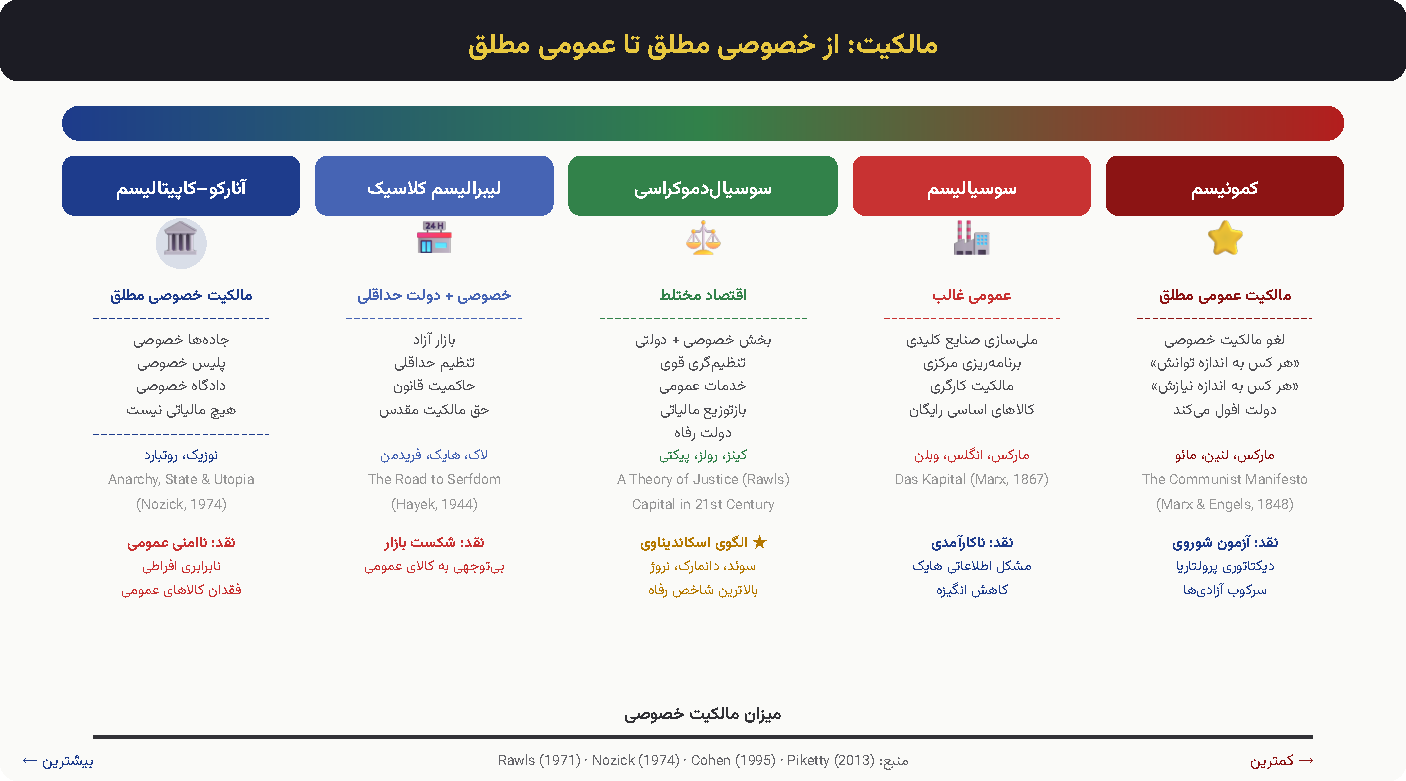
\includegraphics[width=\linewidth]{figures/infographic-property.pdf}
  \caption{طیف مالکیت از آنارکو–کاپیتالیسم تا کمونیسم}
  \label{fig:property}
\end{figure}

\begin{comparebox}[سه نظریهٔ کلاسیک مالکیت]
\begin{center}
\resizebox{\columnwidth}{!}{%
\begin{tikzpicture}[
    node distance=0.4cm,
    box/.style={
      rectangle, rounded corners=4pt,
      minimum width=3.5cm, minimum height=2.6cm,
      align=center, text width=3.3cm,
      draw, inner sep=6pt, font=\small
    }
]
  \node[box, fill=RightBlue!10, draw=RightBlue] (locke) {
    \textbf{\textcolor{RightBlue}{\rl{لاک: کار}}}\\[3pt]
    \rl{مالکیت از کار}\\
    \rl{انسان بر کار خود حق دارد}\\[3pt]
    {\footnotesize\en{Two Treatises (1689)}}
  };
  \node[box, fill=CenterGreen!10, draw=CenterGreen,
        right=0.5cm of locke] (hegel) {
    \textbf{\textcolor{CenterGreen}{\rl{هگل: شخصیت}}}\\[3pt]
    \rl{مالکیت تجسم اراده}\\
    \rl{حقوقی بودن = مالک بودن}\\[3pt]
    {\footnotesize\en{Phil. of Right (1820)}}
  };
  \node[box, fill=LeftRed!10, draw=LeftRed,
        right=0.5cm of hegel] (marx) {
    \textbf{\textcolor{LeftRed}{\rl{مارکس: استثمار}}}\\[3pt]
    \rl{مالکیت ابزار سلطه}\\
    \rl{ارزش اضافی از کارگر}\\[3pt]
    {\footnotesize\en{Das Kapital (1867)}}
  };
  \node[box, fill=GoldAccent!10, draw=GoldAccent,
        right=0.5cm of marx] (nozick) {
    \textbf{\textcolor{GoldDark}{\rl{نوزیک: استحقاق}}}\\[3pt]
    \rl{مالکیت اکتسابی عادلانه}\\
    \rl{انتقال داوطلبانه}\\[3pt]
    {\footnotesize\en{Anarchy, State (1974)}}
  };
\end{tikzpicture}%
}
\end{center}
\end{comparebox}

\ornamentalrule

% ─────────────────────────────────────────────────────────────────
\section*{۶. رویکرد به دموکراسی}
% ─────────────────────────────────────────────────────────────────

\begin{figure}[H]
  \centering
  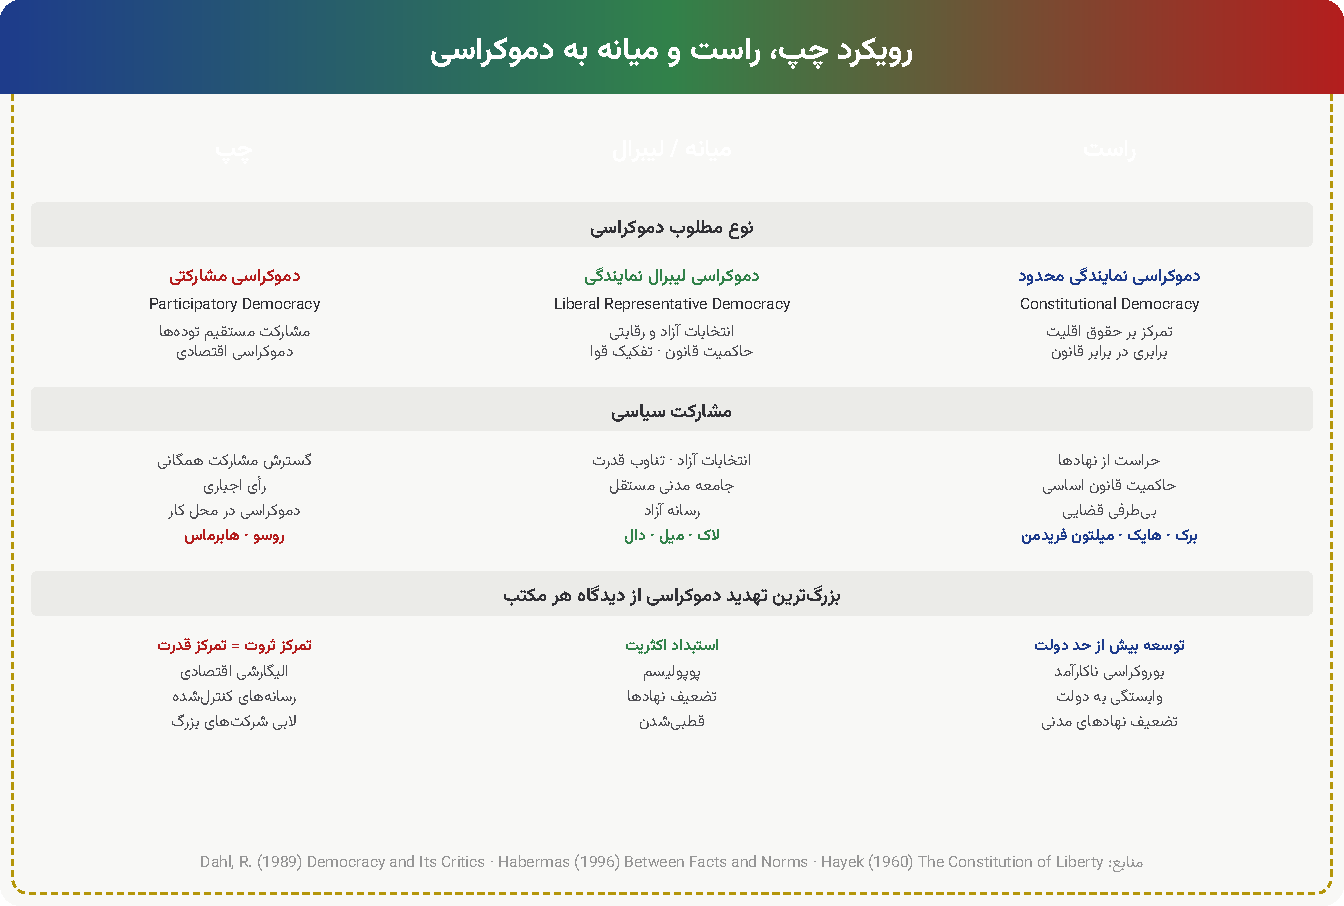
\includegraphics[width=\linewidth]{figures/infographic-democracy.pdf}
  \caption{رویکرد چپ، میانه و راست به مفهوم و انواع دموکراسی}
  \label{fig:democracy}
\end{figure}

\begin{defbox}[انواع دموکراسی و ترجیحات هر مکتب]
\begin{itemize}[leftmargin=*, itemsep=5pt]

  \item \leftkw{چپ — دموکراسی مشارکتی:}
  بر مشارکت مستقیم شهروندان تأکید دارد.
  \person{روسو} (ارادهٔ عمومی) و \person{هابرماس}
  (دموکراسی گفتگویی) از پیشگامان‌اند.\\
  {\small\en{Habermas (1996),
  \textit{Between Facts and Norms}.}}

  \item \centerkw{میانه — دموکراسی لیبرال نمایندگی:}
  \person{دال}، \person{شومپتر} و \person{لاک} پایه‌گذاران این سنت‌اند.
  \person{شومپتر} دموکراسی را «رقابت نخبگان برای کسب آرای مردم» تعریف کرد.\\
  {\small\en{Schumpeter (1942),
  \textit{Capitalism, Socialism and Democracy}.}}

  \item \rightkw{راست — دموکراسی قانون اساسی محدود:}
  \person{هایک}، \person{برک} و \person{مدیسون} بر خطر
  «استبداد اکثریت» هشدار دادند.\\
  {\small\en{Hayek (1960), \textit{The Constitution of Liberty}.}}

\end{itemize}
\end{defbox}

\ornamentalrule

% ─────────────────────────────────────────────────────────────────
\section*{۷. عدالت جبرانی}
% ─────────────────────────────────────────────────────────────────

\begin{figure}[H]
  \centering
  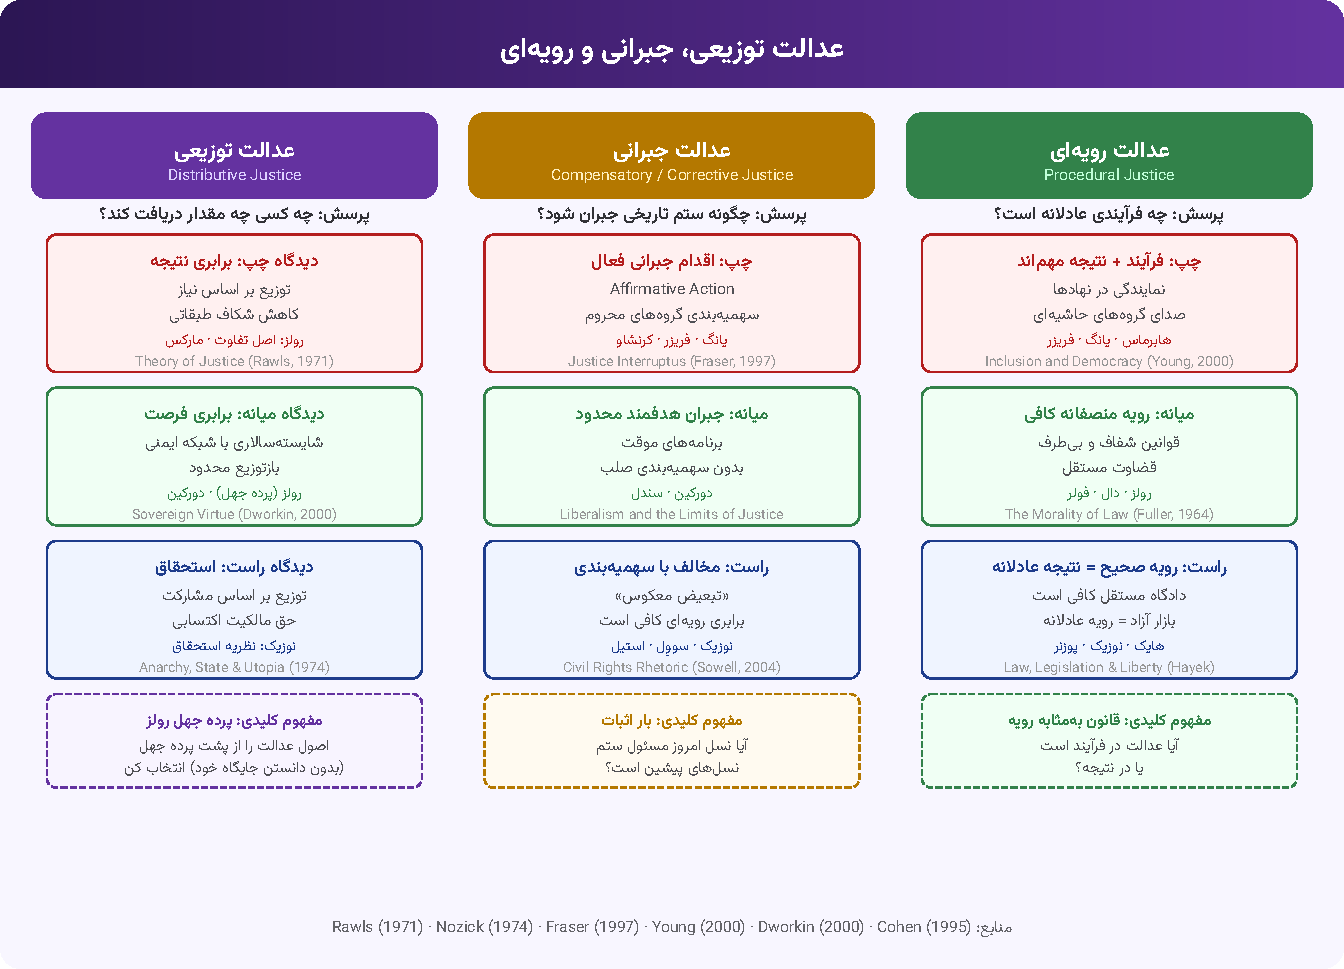
\includegraphics[width=\linewidth]{figures/infographic-justice.pdf}
  \caption{سه گونهٔ عدالت: توزیعی، جبرانی و رویه‌ای}
  \label{fig:justice}
\end{figure}

\begin{defbox}[پرده جهل رولز]
\begin{center}
\resizebox{\columnwidth}{!}{%
\begin{tikzpicture}[every node/.style={font=\small}]
  \fill[DarkGray!80, rounded corners=6pt]
       (0,0) rectangle (12,3.8);
  \fill[DarkGray!40, rounded corners=4pt]
       (0.2,0.2) rectangle (5.8,3.6);
  \fill[DarkGray!40, rounded corners=4pt]
       (6.2,0.2) rectangle (11.8,3.6);
  \node[font=\bfseries\large, text=white] at (6,1.9)
       {\rl{پرده جهل}};
  \node[text=white!80, align=center, font=\footnotesize] at (3,2.8)
       {\rl{نمی‌دانی:}};
  \node[text=white!70, align=center, font=\footnotesize] at (3,2.2)
       {\rl{• ثروت خانواده}};
  \node[text=white!70, align=center, font=\footnotesize] at (3,1.7)
       {\rl{• استعداد فطری}};
  \node[text=white!70, align=center, font=\footnotesize] at (3,1.2)
       {\rl{• نژاد و جنسیت}};
  \node[text=white!70, align=center, font=\footnotesize] at (3,0.7)
       {\rl{• جایگاه اجتماعی}};
  \node[text=white, align=center, font=\footnotesize] at (9,2.8)
       {\rl{چه اصولی انتخاب می‌کنی؟}};
  \node[text=GoldLight, align=center, font=\footnotesize] at (9,2.2)
       {\rl{• آزادی برابر برای همه}};
  \node[text=GoldLight, align=center, font=\footnotesize] at (9,1.7)
       {\rl{• برابری فرصت عادلانه}};
  \node[text=GoldLight, align=center, font=\footnotesize] at (9,1.2)
       {\rl{• اصل تفاوت}};
  \node[text=GoldLight!80, align=center, font=\footnotesize] at (9,0.7)
       {\en{Rawls, 1971}};
\end{tikzpicture}%
}
\end{center}
\mediumspace
\person{جان رولز} در \book{نظریهٔ عدالت} (۱۹۷۱) استدلال کرد
که اصول عادلانه آن‌هایی‌اند که انسان‌ها پشت «پردهٔ جهل» انتخاب می‌کنند.
\end{defbox}

\ornamentalrule

% ─────────────────────────────────────────────────────────────────
\section*{۸. مسئولیت فردی در برابر اجتماعی}
% ─────────────────────────────────────────────────────────────────

\begin{figure}[H]
  \centering
  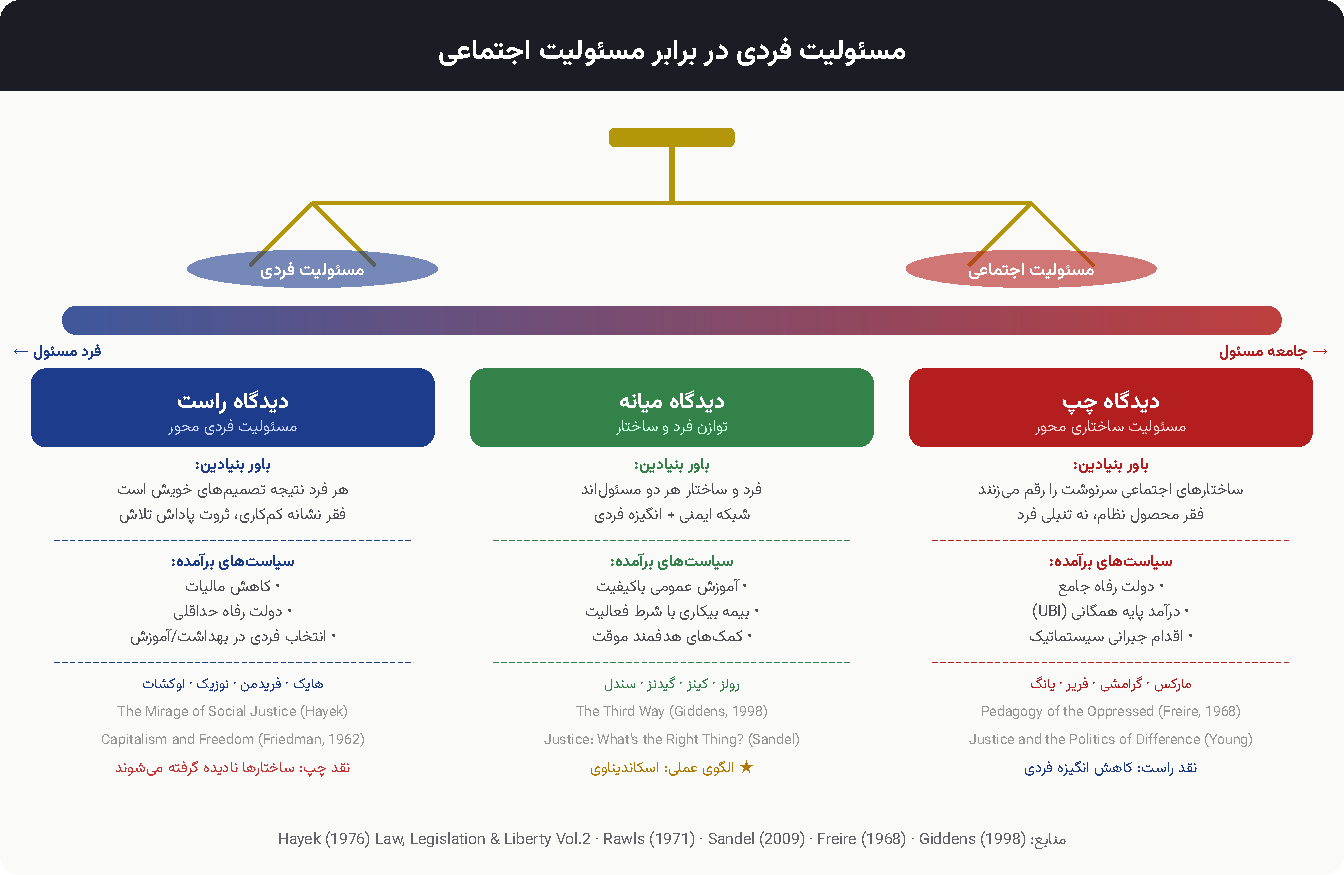
\includegraphics[width=\linewidth]{figures/infographic-responsibility.pdf}
  \caption{تقابل مسئولیت فردی و اجتماعی}
  \label{fig:responsibility}
\end{figure}

\ornamentalrule

% ─────────────────────────────────────────────────────────────────
\section*{۹. تقابل‌های اقتصادی}
% ─────────────────────────────────────────────────────────────────

\begin{figure}[H]
  \centering
  
\includegraphics[width=\linewidth]{figures/infographic-economy.pdf}
  \caption{مقایسهٔ رویکردهای اقتصادی در شش حوزه}
  \label{fig:economy}
\end{figure}

\begin{historybox}[پیکتی و بازگشت نابرابری]
\person{توما پیکتی} در \book{سرمایه در قرن بیست‌ویکم} (۲۰۱۳)
با داده‌های سیصدساله نشان داد:
\[
  r > g \implies \text{تمرکز ثروت افزایش می‌یابد}
\]
راه‌حل: مالیات تصاعدی جهانی بر ثروت.\\[4pt]
{\small\en{Piketty (2013),
\textit{Capital in the Twenty-First Century}, Harvard UP.}}
\end{historybox}

\ornamentalrule

% ─────────────────────────────────────────────────────────────────
\section*{۱۰. جدول جامع تقابل‌ها}
% ─────────────────────────────────────────────────────────────────

% FIXED: longtable با ستون‌های کوچک‌تر برای جلوگیری از overfull hbox
\begin{longtable}{
    >{\columncolor{DarkGray!8}\raggedleft\arraybackslash}p{2.8cm}
    >{\raggedright\arraybackslash}p{3.4cm}
    >{\raggedright\arraybackslash}p{3.4cm}
    >{\raggedright\arraybackslash}p{2.8cm}
    >{\raggedright\arraybackslash}p{2.4cm}
  }

\rowcolor{DarkGray!25}
\textbf{حوزه} &
\textbf{\textcolor{LeftRed}{چپ}} &
\textbf{\textcolor{CenterGreen}{میانه}} &
\textbf{\textcolor{RightBlue}{راست}} &
\textbf{منبع}
\\\hline
\endfirsthead

\rowcolor{DarkGray!25}
\textbf{حوزه} &
\textbf{\textcolor{LeftRed}{چپ}} &
\textbf{\textcolor{CenterGreen}{میانه}} &
\textbf{\textcolor{RightBlue}{راست}} &
\textbf{منبع}
\\\hline
\endhead

\hline
\endlastfoot

% اقتصادی
\rowcolor{RightBlue!6}
\multicolumn{5}{r}{
  \textbf{\textcolor{RightBlue}{\rl{▸ اقتصادی}}}}
\\\hline

مالکیت &
مالکیت اجتماعی &
اقتصاد مختلط &
مالکیت خصوصی &
\en{\footnotesize Nozick (1974)}
\\\hline

مالیات &
تصاعدی شدید &
تصاعدی معتدل &
مسطح یا حداقل &
\en{\footnotesize Piketty (2013)}
\\\hline

دستمزد &
حداقل زیستی بالا &
حداقل ملی &
بازار تعیین کند &
\en{\footnotesize Stiglitz (2012)}
\\\hline

تجارت &
حمایت داخلی &
تجارت آزاد + استانداردها &
آزادسازی کامل &
\en{\footnotesize Ricardo (1817)}
\\\hline

نابرابری &
تهدید دموکراسی &
معتدل قابل قبول &
انگیزه‌بخش &
\en{\footnotesize Rawls (1971)}
\\\hline

% سیاسی
\rowcolor{LeftRed!6}
\multicolumn{5}{r}{
  \textbf{\textcolor{LeftRed}{\rl{▸ سیاسی}}}}
\\\hline

دموکراسی &
مشارکتی &
لیبرال نمایندگی &
قانون اساسی محدود &
\en{\footnotesize Habermas (1996)}
\\\hline

نقش دولت &
هدایت‌گر &
تسهیل‌گر &
حداقلی &
\en{\footnotesize Hayek (1944)}
\\\hline

آزادی &
آزادی مثبت &
هر دو &
آزادی منفی &
\en{\footnotesize Berlin (1969)}
\\\hline

نظم سیاسی &
تغییر بنیادین &
اصلاح تدریجی &
حفظ سنت‌ها &
\en{\footnotesize Burke (1790)}
\\\hline

ملت‌گرایی &
انترناسیونالیسم &
همکاری + حاکمیت &
ناسیونالیسم &
\en{\footnotesize Walzer (1983)}
\\\hline

% اجتماعی
\rowcolor{CenterGreen!6}
\multicolumn{5}{r}{
  \textbf{\textcolor{CenterGreen}{\rl{▸ اجتماعی}}}}
\\\hline

آموزش &
عمومی رایگان &
عمومی باکیفیت &
رقابتی &
\en{\footnotesize Dewey (1916)}
\\\hline

بهداشت &
عمومی جهانی &
بیمه اجباری &
بازار رقابتی &
\en{\footnotesize Beveridge (1942)}
\\\hline

محیط زیست &
مقررات سخت &
مالیات کربن &
نوآوری بازار &
\en{\footnotesize Pigou (1920)}
\\\hline

جرم &
علل اجتماعی + اصلاح &
توانبخشی + بازدارندگی &
مجازات + مسئولیت فردی &
\en{\footnotesize Foucault (1975)}
\\\hline

مهاجرت &
مرزهای باز &
تنظیم‌شده &
کنترل سخت &
\en{\footnotesize Carens (1987)}
\\\hline

% عدالت
\rowcolor{GoldAccent!10}
\multicolumn{5}{r}{
  \textbf{\textcolor{GoldDark}{\rl{▸ عدالت}}}}
\\\hline

عدالت توزیعی &
برابری نتیجه &
برابری فرصت &
استحقاق &
\en{\footnotesize Rawls/Nozick}
\\\hline

عدالت جبرانی &
اقدام مثبت فعال &
جبران هدفمند &
مخالف سهمیه‌بندی &
\en{\footnotesize Fraser (1997)}
\\\hline

مسئولیت &
ساختار اجتماعی &
فرد + ساختار &
مسئولیت فردی &
\en{\footnotesize Sandel (2009)}
\\\hline

\caption{جدول جامع تقابل‌های موضوعی در ۱۸ حوزه}
\label{tab:comprehensive}
\end{longtable}

\vspace{6pt}

\begin{questionbox}
\begin{enumerate}[leftmargin=*, itemsep=8pt]
  \item اگر «پشت پردهٔ جهل» رولز قرار داشتید،
        کدام نظام توزیع ثروت را انتخاب می‌کردید و چرا؟

  \item آیا دموکراسی مشارکتی چپ و دموکراسی قانون اساسی راست
        می‌توانند با یکدیگر ترکیب شوند؟

  \item پیکتی نشان داد $r > g$؛ آیا این به معنای
        ناپایداری ذاتی سرمایه‌داری است؟

  \item مرز میان «آزادی منفی» و «آزادی مثبت» کجاست؟

  \item استروم نشان داد جوامع بدون دولت و بازار می‌توانند
        منابع مشترک را مدیریت کنند.
        این یافته چه چالشی برای هر دو طیف ایجاد می‌کند؟
\end{enumerate}
\end{questionbox}